The line \begin{align}\myvec{-m&1}\vec{x} &= c \end{align}meets it at the point $\vec{P}$ =\myvec{-1\\2} Since, \begin{align}
\vec{P}-\vec{0} = \vec{P}\
\end{align} is the normal vector, where $\vec{0}$ is the origin, then 
\begin{align}
\vec{m}&=\myvec{1\\m}\end{align} is the direction vector, Hence
\begin{align}\vec{m}^T\vec{P}&=0
\end{align}
\begin{align}
\implies\myvec{1&m}\myvec{-1\\2}&=0\notag
\\\implies(-1+2m) &= 0\notag\\
\implies m&=\frac{1}{2}\label{eq:solutions/line_plane/43/1}
\end{align}
 now, the line
 \begin{align}\myvec{-m&1}\vec{x}&=c\notag\end{align} meets it at the point
 $\vec{P}$=\myvec{-1\\2}\notag and using the value of m from \ref{eq:solutions/line_plane/43/1} we get,
\begin{align} 
\myvec{\frac{-1}{2}&1}\vec{P} &=c\notag\\
\implies\myvec{\frac{-1}{2}&1}\myvec{-1\\2} &=c\notag\\
\implies c&=\frac{5}{2}
\end{align}
Hence, the value of m and c are obtained as
\begin{align}
  m=\frac{1}{2} , \  c=\frac{5}{2}\end{align}
  respectively.
See Fig. \ref{fig1:solutions/line_plane/43/}.
\begin{figure}[!ht]
\centering
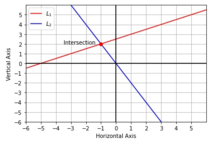
\includegraphics[width=\columnwidth]{./solutions/line_plane/43/Assignment1 plot.png}
\caption{Perpendicular Lines crossing}
\label{fig1:solutions/line_plane/43/}
\end{figure}  
        
    
        
        
        
        
        
        
   


















